\documentclass[thesis.tex]{subfiles}
\begin{document}
\chapter{Introduction}

%\todo{%
%  This chapter should introduce:
%  \begin{itemize}
%  \item Introduce the thesis.
%  \item State the main contributions.
%  \end{itemize}
%
%  We should also ask \emph{what is the thesis of the thesis} which is a fiddly
%  way of asking what are we trying to prove with this document?
%}

\begin{figure}
  \centering
  \includegraphics[width=\linewidth]{figures/mobile-ecosystem.png}
  \caption{Interactions between surrounding the use of mobile devices.}
  \label{fig:mobile-ecosystem}
\end{figure}

Mobile devices are ubiquitous, yet the relationships between their users, and
the environment they run in is often vague. Users have preferences,
companies have policies, and stores have terms; but the precise trust
relationships are often hidden in informal, or natural language, descriptions of
each.

As the devices have become more powerful there has been an increasing wish to
control the devices. Companies expect devices to follow their corporate policies
within their networks and trust users to abide by their policies as well as use
tools to enforce some aspects of them. Some user's may have reservations about
what data apps can get access to and wish to restrict their access. User's may rely on
stores to vet the apps they sell, but will likely not know (or necessarily care)
precisely how the store checked the app.

These devices exist with in the \emph{mobile ecosystem}: which we define as
\textbf{the interactions surrounding the use of smart phones and tablet
computers}. Figure~\ref{fig:mobile-ecosystem} shows some of the relationships
between devices, their users and their preferences, the stores, companies and
all these principal's policies. Users have phones or other mobile devices. They
may own personal devices or have a company one. They may have their own
preferred ways of using the device, or they have to follow policies written
by their employer. They download apps, written by developers from app stores,
all with their own policies and some of the stores may delegate some aspects of
their quality control to external vetting software.

Prior work has focused on how we can check and enforce ever more sophisticated
policies and ever finer controls. This thesis asks a different question:
\textbf{how can we capture the informal policies and trust relationships
surrounding the mobile ecosystem and use formal languages to model and examine
them?} We ask how we can tie the top-level goals in the natural language
policies and preferences to the tools used to implement them? How can we compare
different policies and highlight similarities and differences between them
precisely?

\section{The Need For Policies}

As mobile devices are increasingly capable and hold ever-increasing amounts of
information there is a need from users and businesses to manage how the devices
behave. Employees now bring their mobile devices to work and use them to access
company email and documents. In response to this companies publish mobile device
policies that describe how the devices should be used within the company. These
policies vary in terms of formality. A user may never write their privacy
preferences in a formal language, but they may make decisions guided by them.
For example which apps to install and which to avoid. They may make decisions
based on what their friends have told them, or what a review said about the app.
They may also use \ac{MDM} software, tools which allow companies to configure
mobile devices remotely, to enforce the policies. If a company wishes to use an
app for business purposes there may be regulation they need to follow, such as
\ac{HIPAA}.

A key aspect of the mobile ecosystem is \emph{delegation}. The user of a mobile
device (typically) first logs on to a Google or Apple account before using the
device, which retrieves all their data. Rather than keep account information
locally the app may prompt the user to log in and delegate to a third-party
(such as Google or Facebook) to manage the account ID. When using these
authentication services there are trust relationships between the authentication
services, the users, and the apps they are authenticating with. Capturing these
policies can help clarify the precise terms for authentication and who is
trusted to make what decisions. For example an app might trust Google to manage
accounts. Google will only authorize a user if the user has authorized the app,
and will only allow the app access to the data the user has explicitly
authorized:
\begin{lstlisting}
'app' says 'google' can-say 
  'app' canLink(User:U, Account:A).

'google' says App:A canLink(User:U, Account:Acc)
  if U hasAuthorized(A),
     U hasAccount(Acc).

'google' says User:U can-say U hasAuthorized(App:A)
  if U isAuthenticatedWith(Token),
     Token isValid.

'google' says User:U can-say App:A canAccess(Data:D)
  if D isOwnedBy(U).
\end{lstlisting}

Users may install apps manually themselves, but they might use one or
more app stores to provide them with apps.  They trust these app
stores to provide them with \emph{good and safe} apps, and delegate
the checking of them to the store.  Whereas a user might once have
done the check themselves (or at least delegated to an \ac{AV} package
on their computer) now the responsibility is handed to the stores.
Furthermore all software comes signed either by the developer who
created it (in the case of Google's Play Store), the store that sold
it (in the case of Amazon's app store) or both (Apple's App Store).  A
store may delegate to a third-party app vetting service to determine
what apps are safe (Yandex and Aptoide stores), or use their own
in-house teams.

Users recommend apps to each other. Alice, for example, may trust Bob to tell
her which apps are good.
%
\begin{lstlisting}
'alice' says 'bob' can-say App:A isGood.
\end{lstlisting}
%
Some may consider what apps they want to use on their phone and come up with
informally applied personal policies that describe how they want to use them.
They may never write these policies down, but they might take the form of
preferences that influence the apps they choose, by capturing these we can start
to examine and compare policies as well as potentially enforcing them. For
example Bob may be willing to recommend any app by Nintendo:
%
\begin{lstlisting}
'bob' says App:A isGood
  if A isGame,
     A hasDeveloper('nintendo').
\end{lstlisting}
%
Bob might trust reviews and review sites to give him an idea of an app's quality. 
%
\begin{lstlisting}
'bob' says App:A isGood
  if A hasReviewScore(N)
  where N > 60.
 
'bob' says 'metacritic' can-say
  App:A hasReviewScore(Percent:N).
\end{lstlisting}
%
Bob might also recommend an app based on its app store categorization and its permissions.
%
\begin{lstlisting}
'bob' says App:A isGood
  if A hasCategory('flashlight'),
     A hasPermissions(P)
  where ! contains(P, 'INTERNET').
\end{lstlisting}

They allow their employers to say how they should their devices, who
may in turn delegate to IT departments, to write rules, which may
delegate back to the users to state what rules they're willing to
follow.

A company looking to control their employee's mobile devices at work might write
a \ac{BYOD} policy. They might also use \ac{MDM} software to control some
aspects of their devices. The company might write these with varying degrees of
formality but often they are written using natural language. This adds vagueness
and can lead to confusion as to how a policy should be implemented. By
describing the policy in a formal language we can start to express the policy
more rigorously. We can start to make comparisons between users, and with rules
for checking the policy start to help the user to make decisions more
accurately, or measure the extent a user follows their stated policy. Using
formal languages we can model the policies precisely, helping clarify their
meanings and make precise comparisons between different policies. We can tie the
rules in the \ac{BYOD} policies, for example, to the \ac{MDM} tools used to
implement them.

If a company needs to use apps which conform with a policy such as
\ac{HIPAA} they could use static analysis tools to check for some
aspects of the policy.  Perhaps the company might use
Mallodroid~\cite{fahl_why_2012} to detect when data is sent
unencrypted.  
%
\begin{lstlisting}
'company' says Employee:E canUse(App:A)
  if A isHIPAAConformant
  where
    mallodroidCheckSafe(A) = True;
\end{lstlisting}
%
It is important, however, not to confuse the tools and
techniques we might use to implement parts of a policy with the end
goal of ensuring that the policy is followed.  A formal language that
lets us sever the policy from its implementation can help us
understand the policy precisely, and then show precisely how the
policy is checked.  It lets us see what rules from the policy are
checked for by which tools, and identify gaps where the policy is not
being checked sufficiently.

These trust relationships and delegations permeate the entire mobile
ecosystem.  They represent an important aspect of the ecosystem that a
policy language should catch in order to adequately describe the
relationships and policies within it.

One approach to designing a policy language is to base it on a logic of
authorization. Authorization logics~\cite{abadi_calculus_1991} describe rules
for deciding when an action is permitted, and reasoning about why that action
was allowed. A common use case for these logics is building access control
systems. A user is allowed to read a file if he or she has the appropriate
permissions. In applying logics of authorization to policy language the policy
language describes who can access what, but the authorization logic gives a
formal description of how we make that decision. We want to use a policy
language to describe the trust relationships in the mobile ecosystem.

\section{History of Mobile Devices}

\begin{figure}\sffamily\scriptsize
  \centering
  \begin{chronology}[5]{1993}{2017}{\textwidth}
    \event{1993}{Apple Newton}
    \event{1994}{IBM Simon}
    \event{1996}{Palm Pilot}
    \event{1998}{Symbian}
    \event{1999}{BlackBerry}
    \event{2000}{\stackanchor{Java Micro Edition and Windows Mobile}{First mobile virus (Timofonica) discovered}}
    \event{2003}{Nokia N-Gage}
    \event{2005}{iOS released, Commwarrior-A worm discovered}
    \event{2008}{Android, iPhone and App Store}
    \event{2010}{\stackanchor{Windows Mobile becomes Windows Phone}{iPad}}
    \event{2012}{Symbian discontinued}
    \event{2013}{Sailfish OS}
    \event{2015}{\stackanchor{Windows Phone discontinued}{non-Android BlackBerry devices discontinued}}
  \end{chronology}
  \caption{Timeline of mobile device developments.}
  \label{fig:timeline-mobile}
\end{figure}

Some of the earliest mobile devices were the \acp{PDA} devices such as Apple's
Newton and the Palm Pilot. They were portable miniature computers designed to
store personal information, calendars and notes. Developers could program
additional apps for them. In the 1990s mobile phones were just portable
telephones, but with the IBM Simon in 1994 these devices started to have some of
the functionality of the \ac{PDA}, becoming what would later be called a
\emph{smart phone}. These early smart phones had a telephone connection, unlike
the \acp{PDA}. The earliest smart phones could access email and fax, as well as
managing personal information, but were somewhat underpowered compared to the
\ac{PDA} devices.

In 1998 the Symbian OS was released. Symbian devices could install apps, written
in C++ or Java (if the phone supported JME). They had cameras, could play music.
They even had early malware which would illicitly send texts to premium rate
numbers. They were the forebears of the \emph{modern} smart phone. They were
also starting to become affordable, with the lowest end models starting to be
affordable. Devices like Nokia's N-Gage were marketed directly towards children
and teenagers and had games users could buy for their devices. Others, such as
the BlackBerry were marketted towards business users.

By the mid-2000s the devices were ubiquitous. Windows Mobile was released in
1999, and the first version of iOS was released. Users could browse the web, and
send each other pictures. The first modern app store was released for iOS in
2008\footnote{Earlier attempts existed but resembled Linux package managers.}.
With increasing amounts of personal information available on these devices
malware authors started to take note. The first mobile virus was found in 2000
which sent text messages\footnote{The Timofonica virus infected Windows PCs to
send text messages via a web based SMS gateway. It was not harmful, only
irritating.}, but by 2005 the self-replicating Commwarrior worm was discovered
that ran entirely on smartphones.

Despite increasing amount of malware, in a blog post from 2006 for Symantec,
Chien noted that adware and privacy invading apps were likely to be a bigger
threat~\cite{eric_chien_spyware_2006}. These would likely require new controls to
help manage user's privacy preferences, an idea that would be picked up by the
fine-grained permissions research (see \autoref{sec:fine-grained-permissions}).

\begin{quote}
  ``While threats exist and are actively spreading, we are probably
  still years away from the situation we have with the Microsoft Windows
  [$\cdots$] We have already seen spyware applications for mobile devices
  (e.g. Spyware.Flexispy) that can monitor activities on the mobile
  device and then send them to a remote server. [$\cdots$] Just as
  worrying is the fact that the adware market is just beginning to take
  notice of mobile devices. Already some Bluetooth advertising schemes
  have been tested, where a bus stop is outfitted with a device that
  just spams out messages via Bluetooth.

  [$\cdots$]
  
  So, while worms and Trojans already exist for the mobile
  platforms, spyware and adware applications are just now gaining a
  foothold in the mobile device space. Spyware and adware pose a
  potentially large security issue in the near future, as the companies
  that produce such applications are less affected by the natural
  limiting factors.''
\end{quote}

\subsection{Modern Mobile Devices}

In 2008 Apple released the first iPhone, and shortly after Google
released the Android OS.  Symbian released its final version in
2012, and was replaced by Android as the dominant OS on most devices.  

Android and iOS differ from past efforts, and conventional desktop OSs, as they
made it far harder to run arbitrary unvetted programs. Apple's devices cannot
run code that Apple has not signed or install software from outside of its App
Store, which Apple controlled. Android devices offer a similar app marketplace,
but where there is less checking of individual
apps~\cite{oberheide_dissecting_2012}. Whilst Android users can install software
from other sources, the option is hidden by default. As well as restrictions to
software, the OSs are also better hardened. Devices no longer have all powerful
\emph{root} account, and APIs are provided to allow controlled access to
sensitive data and restrict malicious behaviors; such as stopping SMSs being
sent programatically to premium rate accounts.

Mobile devices store an increasing amount of personal data about their users.
They contain address books, records of phone calls, and GPS logs of where their
users had been. With iOS and Android users have become more aware about privacy
issues with their devices, in part because of increased media coverage of
privacy issues.

A survey in 2012 by Chin~et~al{.} found that users were more concerned about
privacy on their mobile devices, than on their
laptops~\cite{chin_measuring_2012}. They found that users of a smartphone were
more likely to install an app that came recommended from a friend, was popular
or was free. To subsidize the cost of producing free apps, and to better
understand how users used their apps, some developers have added adware and
tracking libraries to their apps, as predicted by Chen. These libraries add
crash and error tracking, as well as collecting personal data to be sold to
advertisers to subsidize the app's price~\cite{seungyeop_han_study_2012}.

This dynamic between users who were increasingly concerned about their
privacy and apps which were increasingly privacy invading has lead to many papers proposing finer privacy
controls~\cite{jeon_dr._2012,beresford_mockdroid:_2011,conti_crepe:_2010,backes_appguard_2013}.  
In general, however, users appear to not understand the how permissions worked~\cite{felt_android_2012}. 

Android and iOS have settled on a model for permissions where users are asked by their
devices if an app can access certain data when it first requests it.
Users can revoke that decision later if they wish.

Android's current \emph{ask on use} permissions model was released in 2015, but
a large number of older Android devices, which cannot control permissions, are
still being used. In June 2016 only 10\% of devices used the latest version of
Android, with around 5\% using a version more than five years old. In contrast 79\% of iOS devices use the latest
OS, 16\% use the previous version and only 5\% use anything
older~\cite{apple_app_2017}. This means that many Android user's cannot benefit
from improved privacy controls.

%\begin{figure}
%\centering
%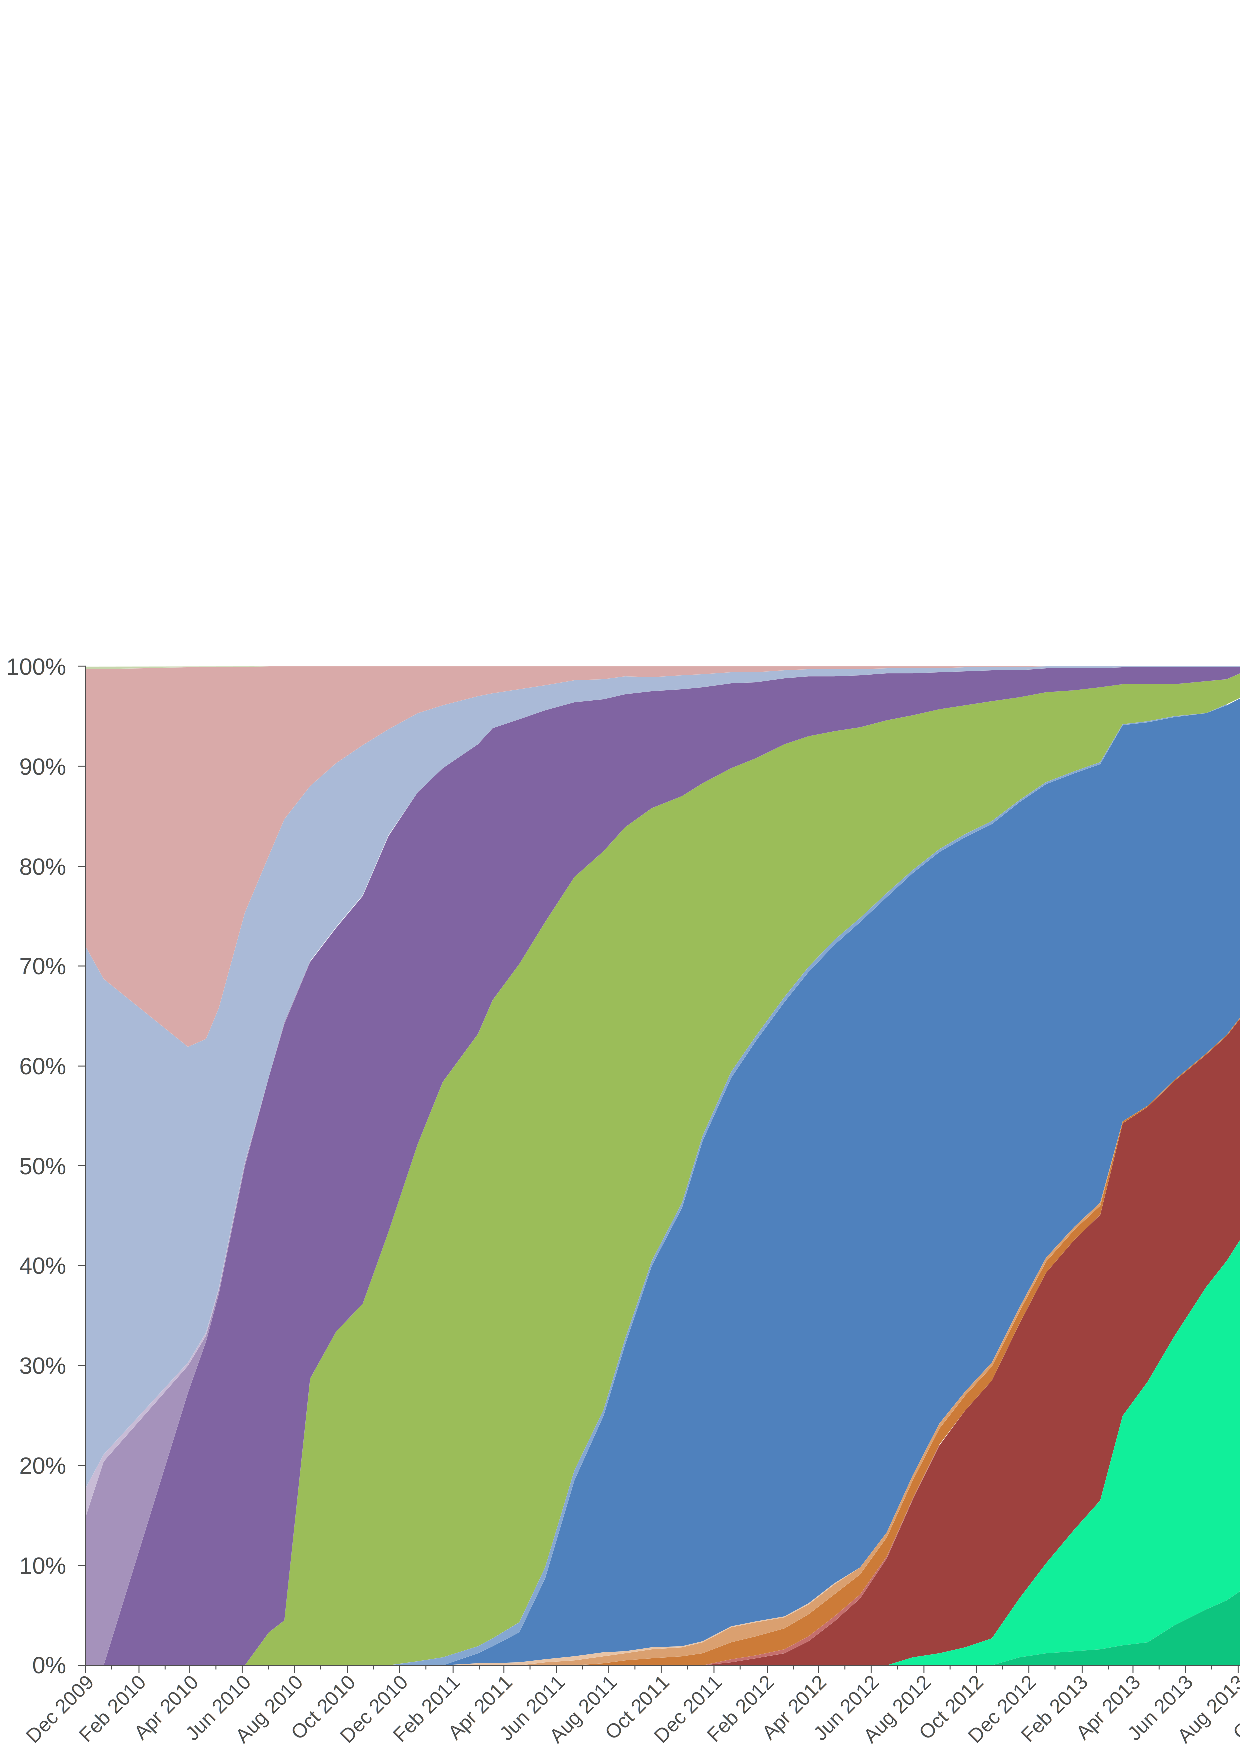
\includegraphics[width=\linewidth]{figures/android-versions.pdf}
%\caption[Historical Android version's distribution.]{Historical Android
%  version's distribution~\cite{erikrespo_android_2017}.}
%\label{fig:android-versions}
%\end{figure}

Mobile devices also store increasingly personal information. Smart watches
record and shared a user's pulse with others. Mobile health apps track and
monitor medical conditions. In the US, the \ac{HIPAA} regulation requires that
healthcare providers transmit medical information securely, but many apps have
basic security problems~\cite{fahl_why_2012}, and many of the healthcare apps
do not handle information securely~\cite{knorr_privacy_2015}.

Software is predominantly distributed through app stores.
To install an app on an early mobile device the user would
download it on a traditional computer and then transfer it to the
mobile, where they could install it using a package manager.  App
stores have made this simpler by allowing users to find
an install apps straight from their device.  Whilst the app store is
the normal method of installing apps, apps can still be downloaded and
installed manually by side-loading on Android or through iTunes for
iOS.

On Android Google's Play Store is often the
default app store but users are free to choose other marketplaces if they wish.
One choice is Amazon's Appstore.  It is the default for Amazon's
Kindle Fire tablets, and has special offers for Amazon customers.
Other marketplaces are regional.  In China, where Google web services
cannot be used, alternative markets such as Qihoo360 and Baidu have
appeared.

%\todo{Introduce how app stores are the primary mechanism for
%distributing software in the ecosystem.  Describe and possibly show
%the interface, and reviews.  Maybe move the marketshare diagram from
%later on into here?  }

%\begin{figure}
%  \centering
%  \includegraphics[width=0.31\textwidth]{figures/store-home.png}
%  \includegraphics[width=0.31\textwidth]{figures/store-app.png}
%  \includegraphics[width=0.31\textwidth]{figures/store-review.png}
%  \caption[Apple's App Store.]{Apple's App Store.  Showing the store's frontpage, an app's page, and its reviews.}
%  \label{fig:appstore}
%\end{figure}
%
%Figure~\ref{fig:appstore} shows Apple's App Store.  Users are first
%presented with featured apps, though they can also browse for apps by
%category, search, or look at \emph{top charts}.  If a user touches an
%app they are presented with more information.  This particular app,
%\emph{Eggggg}, is the free app of the week.  The app's name and
%age-rating (9+) is shown alongside the a link to the app's developer.
%A button is presented for the user to install the app or open it if it
%has already been opened.  Additional information is displayed about
%the app: it will work with Apple's messaging app, and also with their
%Apple TV devices.  The App store editor has, in this case, written a
%note about it describing the app which is displayed prominently.  If
%the user reads down the page a description of the app by the developer
%is also given, as well as screenshots, a changelog, detailed
%information including device compatibility, and a link to the apps
%privacy policy.  This particular app offers in app purchases and the
%user is warned of this prominently on this screen.  A review score is
%also displayed. This app has 4 out of 5 stars based on twelve reviews.
%If the user touches the review tab, they can see more detailed reviews
%by named reviewers.  These can vary in quality (this particular app's
%top reviews are not helpful) and the developer can respond to
%individual reviews.  User's can optionally write a review for the app.

%Precise numbers of apps in different stores is hard to get, but the
%largest stores occassionally give rough
%numbers~(\autoref{fig:app-store-apps}).  Google and Apple's stores
%have (as of the end of 2016) around 2.5 million apps, with Amazon's
%store having considerably less.
%
%\begin{figure}
%  \includegraphics[width=\textwidth]{figures/app-store-apps.pdf}
%  \caption[Reported numbers of different apps on various App marketplaces.]{%
%    Reported numbers of different apps on various App marketplaces. Data taken from~\cite{statista_google_nodate,statista_apple_nodate,statista_amazon_nodate}.}
%  \label{fig:app-store-apps}
%\end{figure}

\section{Publications}

The work described in this thesis builds upon work published in these publications:

\begin{itemize}
%\item \bibentry{hallett_capturing_2017}
\item 
Joseph Hallett and David Aspinall. Capturing Policies for BYOD. In \emph{IFIP Security and Privacy Conference}, 2017
%\item \bibentry{hallett_common_2017}
\item Joseph Hallett and David Aspinall. Common Concerns in BYOD Policies. \emph{In Workshop on Innovations in Mobile Privacy and Security}, April 2017
%\item \bibentry{hallett_specifying_2016}
\item Joseph Hallett and David Aspinall. Specifying BYOD Policies with Authorization Logic. \emph{In PhD Symposium at iFM'16 on Formal Methods. Reykjavik University}, June 2016
%\item \bibentry{hallett_apppal_2016}
\item Joseph Hallett and David Aspinall. AppPAL for Android. \emph{In Engineering Secure Software and Systems. Springer Verlag}, April 2016
%\item \bibentry{hallett_poster:_2015}
\item Joseph Hallett and David Aspinall. Poster: Using Authorization Logic to Capture User Policies in Mobile Ecosystems. \emph{In Symposium on Usable Privacy and Security}, 2015
%\item \bibentry{hallett_towards_2014}
\item Joseph Hallett and David Aspinall. Towards an authorization framework for app security checking. \emph{In Engineering Secure Software and Systems}, 2014
\end{itemize}


\end{document}


%%% Local Variables:
%%% mode: latex
%%% TeX-master: "../ch1"
%%% End:
